\chapter{Application of Markov Chain}
Markov chain Has  numerous application in real life. Let us explore house in this chapter.

\section{Google PageRank}
Before google surfing in the web is very hard, in search engines page was rank by primly on keyword-based algorithms to rank web pages. 
One popular early search engine, called AltaVista, used a ranking algorithm that focused on keyword matching. 
It would examine factors like the frequency of the keyword in the page's content, 
the placement of the keyword (e.g., in titles or headings), and the number of times the keyword appeared in the page's metadata.
Keyword-based algorithm is very easy to misuse. A spam page could boost its ranking
just by including a long list of words repeated over and over again.

In other hand taking the link structure into account led to dramatic improvements
in search engines. As a first attempt, one could rank a page based on how many
other pages link to it. That is, if Page A links to Page B, we consider it a “vote”
for B, and we rank pages based on how many votes they have.
But this is again very open to abuse: a spam page could boost its ranking by creating
thousands of other spam pages linking to it.
And though it may seem democratic
for each page to have equal voting power, an incoming link from a reliable page is
more meaningful than a link from an uninformative page.

To solve this problem Sergey Brin and Larry Page develop a algorithm to rank page
in their search engine Google and named it after Larry Page Google PageRank, 
which was introduced in 1998. Google PageRank ranks
the importance of a page not only by how many pages link to it, but also by the
importance of those pages.

To under stand Google PageRank we consider a smaller version of World Wide Web 
contain only 4 pages connected as shown in \cref{A small Web Containing 4 page}.

\begin{figure}[H]
    \centering
    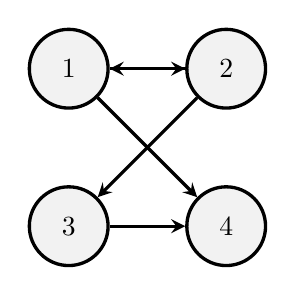
\begin{tikzpicture}[->, >=stealth, auto, very thick, node distance = 2cm, state/.style={circle, draw=black, fill=black!5, very thick, minimum size = 10mm}]
        \node[state] (1) {$1$};
        \node[state] (2) [right of=1] {$2$};
        \node[state] (3) [below of=1] {$3$};
        \node[state] (4) [below of=2] {$4$};

        \path (1) edge [] (2)
            (2) edge [] (1)
            (1) edge [] (4)
            (2) edge [] (3)
            (3) edge [] (4);
    \end{tikzpicture}
    \caption{A small Web Containing 4 page}
    \label{A small Web Containing 4 page}
\end{figure}

Imagine someone randomly surfing the web, starting at some page and 
then randomly click to got from one page to the next (with equal probabilities for
all links on the current page).
 The idea of PageRank is to measure the importance
of a page by the long-run fraction of time spent at that page.

Of course, some pages may have no outgoing links at all, such as page 4 above. When
the web surfer encounters such a page, rather than despairing he or she opens up a
new browser window and visits a uniformly random page. Thus a page with no links
is converted to a page that links to every page, including itself. For the example
above, the resulting transition matrix is

\[
    P =
    \begin{bmatrix}
        0 & 1/2 & 0 & 1/2 \\ 
        1/2 & 0 & 1/2 & 0 \\ 
        0 & 0 & 0 & 1 \\
        1/4 & 1/4 & 1/4 & 1/4
    \end{bmatrix} 
\]

If we start with probability vector 
$ \mathbf{t} = \begin{bmatrix}
    1/4 & 1/4 & 1/4 & 1/4 
\end{bmatrix}  $.\\ 
i.e. every page has equal probability to visit in first state. Then the 2nd step 
probability vector will be 
$\mathbf{t}_{1}= 
    \begin{bmatrix}
        0.1875 & 0.1875 & 0.1875 & 0.4375 
    \end{bmatrix} 
$.\\ 
Now doing $ \mathbf{t}_{2}P $ we get the 3rd step probability vector $ \mathbf{t}_{3} $.
After reputing this process we get.
\[
    \mathbf{t}_{100} \approx \mathbf{t_{101}} = \begin{bmatrix}
        0.2 & 0.2 & 0.2 & 0.4 
    \end{bmatrix} 
\]
Hence it is the stationary probability.

In general let $ M $ be the number of pages on the web, let  $ P $ be the  $ M\times M $
transition matrix of the chain described above, and 
let $ \pi $ be the stationary distribution.
Think of $ \pi_{j} $ as a measure of how important Page $j$ is. 
Hence the equitation 
\[
    \pi_{j}=\sum_{i=0}^{M} \pi_{i}p_{ij}
\]
says that the score of Page $j$ should be based not only on how many other pages link
to it, but on their scores.

It is not clear that a unique stationary distribution exists for this chain, 
since it may not be irreducible and aperiodic. 
Even if it is irreducible and aperiodic, convergence
to the stationary distribution could be very slow since the web is so immense. To
address these issues, suppose that before each move, the web surfer flips a coin
with probability $ \alpha $ of Heads. If Head, the web surfer click to a random 
link from the current page; if Tails, the web surfer teleports to uniformly random \
page. The resulting chain has the \textit{Google transition matrix}

\begin{equation}
    \label{google transition matrix}
    G = \alpha P + (1-\alpha) \frac{J}{M},
\end{equation}

where $ j $ is the  $ M\times M $ matrix of all entries are 1. Note that the row sums 
of $ G $ are 1 and that all are positive, so  $ G$ is valid transition matrix for an 
irreducible, aperiodic Markov Chain. Which means that it has unique stationary 
distribution $ \pi $, called \textit{PageRank} and the chain is converge to it.
 
The choice of $\alpha$ is an important consideration; 
choosing $ \alpha $ close to 1 makes sense to respect the structure of the
web as much as possible, but there is a tradeoff since it turns out that smaller
values of $ \alpha $ make the chain converge much faster. 
As a compromise, the original recommendation of Brin and Page was $\alpha = 0.85$.

PageRank is conceptually nice, but computing it sounds extremely difficult, considering
that that $ \pi G=\pi $ could be a system of 100 equations in 100 billion unknowns.
Instead of thinking of this as a massive algebra problem, we can use the Markov
chain interpretation: for any starting distribution  $ \mathbf{t} $,  
$\mathbf{t}G^{n}\to \pi$ as $ n\to\infty $. And $ \mathbf{t}G $ is is easier to 
compute that it seems at first:
 \[
     \mathbf{t}G = \alpha(\mathbf{t}P) +\frac{1-\alpha}{M}(\mathbf{t}J),
\]
where computing the first term is easy to compute as most element $ P $  is 0 and 
computing the second term is very easy $ \mathbf{t}J $ is a vector of all 1. 
To compute $ \mathbf{t}G^{n} $ by $ (((\mathbf{t}G)G)\ldots) $. After a very long 
iteration of $ n $ if it appear to convergent then we say  it is the approximation
of PageRank.

For the above example 
\[
    \mathbf{t}_{10000}\approx\mathbf{t}_{10001} = 
    \begin{bmatrix}
        0.2004008 & 0.2004008 & 0.2004008 & 0.3987976 
    \end{bmatrix} 
\]
Hence it is approximate Stationary Distribution.
